\chapter{系统软件}

\section{U-boot}

\subsection{背景}
U-Boot 是一个启动引导程序,常见于嵌入式系统中,用于引导 Linux 等操作系统。在本系统的设计中,U-Boot 将作为引导程序,放置在BRAM中;同时,我们根据展示需求,修改了U-boot源码以增加更多功能。

\subsection{移植内容}

\begin{itemize}
    \item 使用 U-boot v2023.07稳定版本
    \item 修改底层驱动,使其支持VGA Console+PS/2键盘输入输出
    \item 添加如图4.1所示的菜单启动界面,能够自动通过网口加载并选择性启动 Linux 或 ucore 操作系统
\end{itemize}

%开始插入图片
\begin{figure}[htb] % htbp代表图片插入位置的设置
\centering %图片居中
%添加图片;[]中为可选参数,可以设置图片的宽高;{}中为图片的相对位置
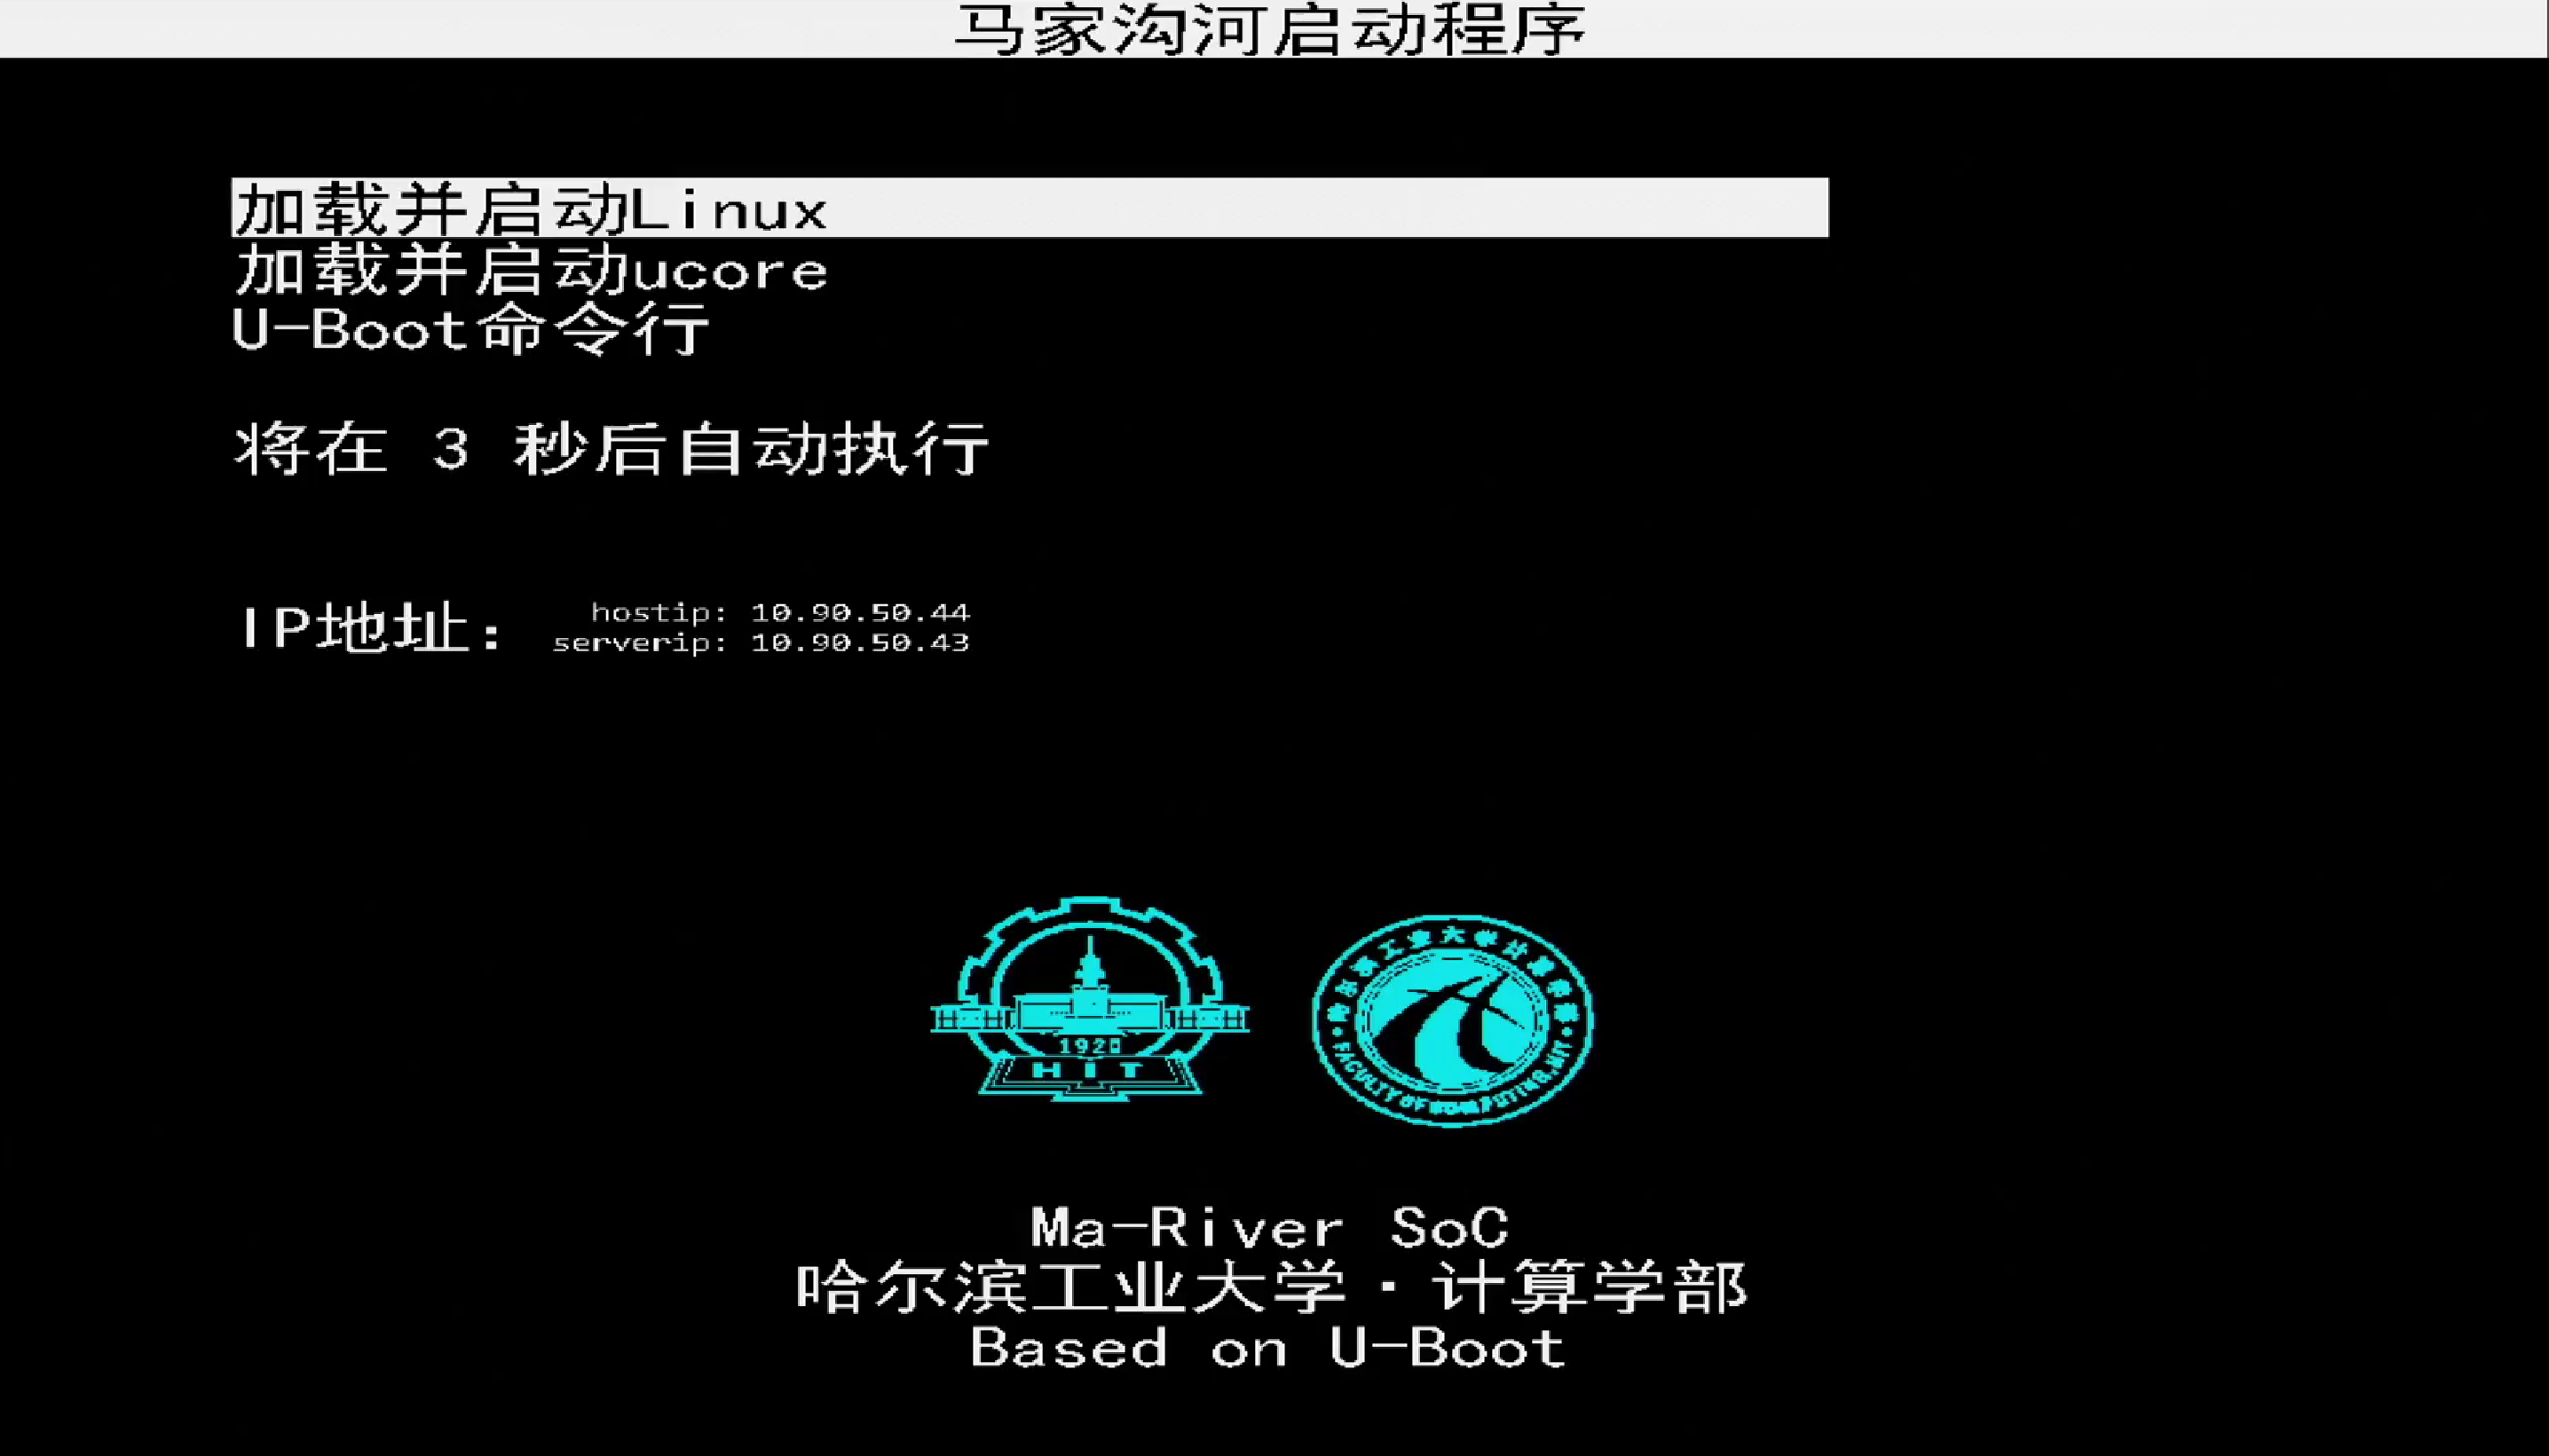
\includegraphics[width=13cm]{img/uboot.png}
\caption{U-Boot菜单启动界面} % 图片标题
\label{pic2} % 图片标签
\end{figure}

\section{ucore}

\subsection{背景}
ucore是清华大学的轻量级教学操作系统。

\subsection{移植内容}
\begin{itemize}
    \item 修改底层驱动,使其支持VGA Console+PS/2键盘输入输出
    \item 在U-Boot启动菜单中增加ucore自启动选项。
\end{itemize}

\section{Linux}
\subsection{背景}
Linux 是最为著名的开源操作系统,有丰富的软硬件支持。我们以最新的稳定版本 Linux v6.4 (2023年6月26日发布)作为基线进行移植。

\subsection{驱动程序}

\subsubsection{LCD驱动}
我们自行实现了LCD驱动,分为3个部分:文本传输,普通图像传输和标准FrameBuffer,它们分别对应/dev/下3个独立的字符设备。文本传输设备通过write在LCD的文本模式下顺序输出字符,类似串口。普通图像传输设备可通过ioctl接受DMA地址实现DMA快速传输\texttt{dma\_sync\_single\_for\_device}清理Cache实现数据同步,这允许了像素数据在传输前可以充分使用Cache,提升处理性能。为减少阻塞,驱动程序对于多个未开始的DMA请求维护一个缓冲,当DMA中断发生时取下一个请求发送给控制器。

\subsubsection{VGA Console驱动}  
我们仿照内核默认的\verb|dummy console|以及自带的\verb|vga console|驱动程序,实现了用于自己VGA控制器的\verb|consw|结构体及文本输出/滚屏/光标设置等的底层接口函数,它们都基于VGA控制器文本模式的操作。我们修改了内核启动代码,将默认Console(\verb|conswitchp|)设置为我们自己的,这样在Linux内核初始化完成后,可直接使用基于我们VGA Console驱动的\verb|tty0|虚拟终端。由于VGA控制器的文本模式仅使用片上存储,不会与CPU竞争内存带宽,相比于常规的基于FrameBuffer的Console实现方式,这可以为系统带来更高的性能。

Linux使用VGA Console的启动效果如图4.2所示。

%开始插入图片
\begin{figure}[htb] % htbp代表图片插入位置的设置
\centering %图片居中
%添加图片;[]中为可选参数,可以设置图片的宽高;{}中为图片的相对位置
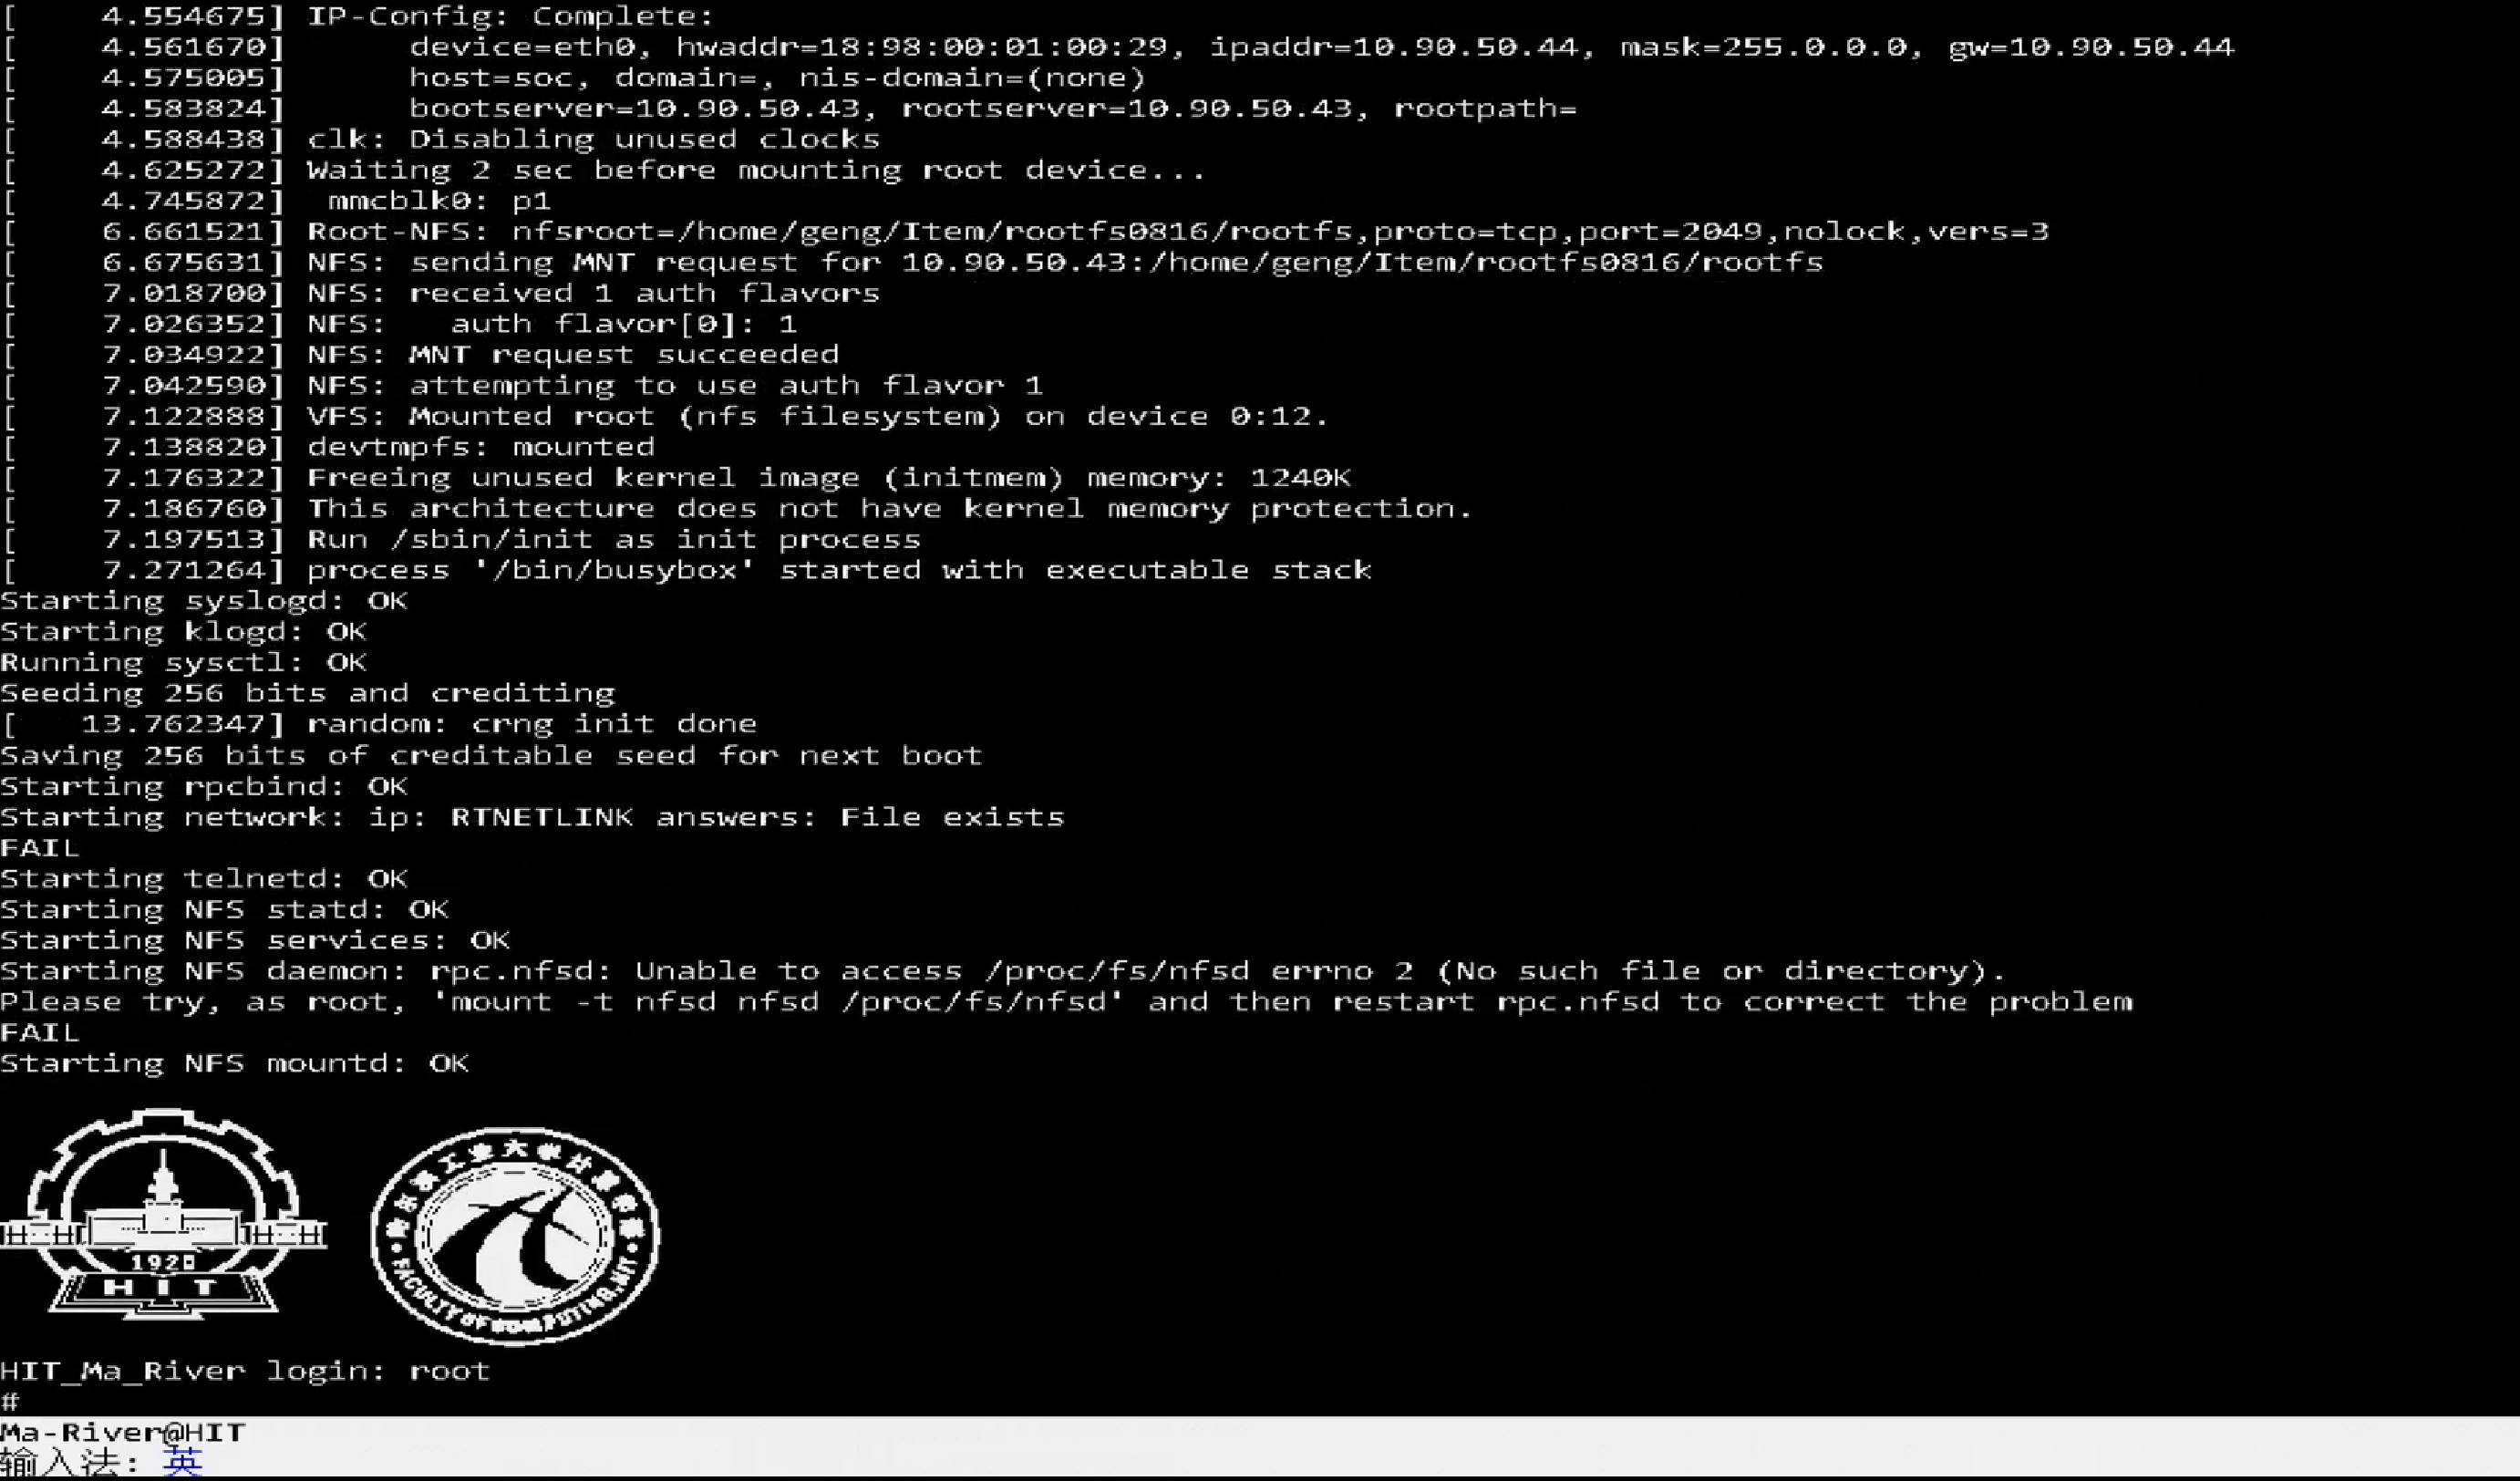
\includegraphics[width=13cm]{img/linux.png}
\caption{Linux启动界面} % 图片标题
\label{pic3} % 图片标签
\end{figure}

\subsubsection{PS/2键盘驱动}
Linux启动后会使用虚拟终端,它的输入最终基于一个完备的input子系统,这给我们自行实现的键盘驱动带来了便利。我们只需要令键盘中断处理程序读取扫描码,通过\texttt{input\_report\_key}向内核的input子系统上报键盘输入事件即可。

\subsubsection{Framebuffer驱动}
为了能够支撑更多GUI应用,我们还为VGA和LCD控制器实现了Framebuffer驱动。Framebuffer驱动的实现包含如下部分:一,开辟一块内存区域,存放每个像素的颜色信息;二,以合适的方式向显示设备传送内存中的颜色信息。
由于我们的VGA控制器和LCD模块本身均采用RGB565颜色格式,故在实现驱动时使用同样的格式进行像素信息的存储,因而每个像素需要2字节空间。
由于我们实现的VGA、LCD控制器均支持DMA,故我们仅需向控制器传送内存区域首地址,由控制器直接进行数据的读取,即可完成图像显示。其中,VGA控制器可自行进行不间断的数据读取;但LCD控制器完成一次数据传输后便会停止,所以我们使用计时器机制,每隔50ms传送一次内存区域首地址,以20Hz刷新率显示图像。

\subsubsection{SD驱动}
由于我们通过AXI QUAD SPI IP核对SD卡进行操作,所以直接使用了该IP核对应的SPI总线驱动;同时,我们也直接使用了Linux内核主线中使用SPI总线的MMC驱动。在设备树中记录设备相关信息后,即可在进入Linux内核后将SD卡分区挂载到目录树中,进行读写操作。

\subsection{用户态组件}
Linux 内核本身并不能提供任何用户态组件,因此我们需要手工编译这一部分。我们选 择了著名的嵌入
式 Linux 开发工具套件 buildroot 来协助完成用户程序的构建。构建过程 中,我们选择了 glibc 作为系统的C/C++ 标准库实现,并使用 busybox 来提供大部分的 命令行工具。由于构建的 rootfs 较大,无法使用
initramfs 等方式直接加载,而 Flash 的读写速度也 较慢并不灵活,因此我们使用 NFS 协议通过网络挂载系
统的根分区。实践证明,在网络稳定的情况下,系统的响应速度并不会受到影响。
我们成功移植了如下内容:
\begin{description}
    \item[GCC] 由于 buildroot 理念在于生成体积更小的根文件系统,所以不支持GCC移植,我们参考linux-from-scratch\footnote{\url{https://www.linuxfromscratch.org/}} 对GCC进行移植,并对glibc以及binutils利用相同方法移植到系统中,此外,由于 Ma-River CPU 实现了FPU,所以在编译时我们添加了支持硬件浮点的选项,经过测试,GCC可以成功编译出浮点指令并成功运行。我们在Ma-River上用移植的GCC编译了小游戏2048,并成功在Ma-River上运行,以此突出我们的移植工作。
    \item[QEMU] 我们成功移植了著名开源项目QEMU,并生成了可以模拟RISC-V架构的系统级模拟器 \text{qemu-system-riscv64} ,但可惜的是实验板内存只有128MB,无法满足系统级模拟器的运行需求。
    \item[Python] 我们移植了Python3,并且添加了数据处理相关的库(numpy,scipy等)。我们还使用Python搭建了简单的http服务器,浏览器可以在局域网中访问板载服务器上的网页。以此证明我们的 CPU 能够在板载资源更充足的情况下运行更加复杂的应用,体现出我们工作的实用性。
    \item[Busybox] 使用Busybox提供大部分命令行工具。
    \item[网络工具] 移植了常用网络工具(ip,ping,wget,nc,ssh)大大提高了后续的移植以及测试工作的效率。
\end{description}

\subsection{新增内容}
\subsubsection{中文支持}
我们在VGA Console和键盘驱动程序的基础上,为Linux终端增加了基本的中文输入输出能力,基于标准的UTF-8编码,不仅可以输入/显示汉字,还可以将文件名等设为中文进行操作。在我们自己实现的CPU及计算机系统上支持中文汉字处理,也是一件颇有意义的事情。

我们的VGA控制器在文本模式下具有二值化图像显示能力,这使得软件理论上可基于字库绘制复杂字符。我们向VGA Console驱动程序中加入了使用Unicode索引的汉字点阵字库(宋体),收录了符合GBK规范的所有汉字。这样驱动程序可在屏幕某位置显示占两格的汉字。我们还对Linux内核中的虚拟终端负责输出字节流解码的部分作出了简要修改,使其不会对汉字对应的UTF-8编码报错,并正确地将汉字对应的Unicode码值传递给底层VGA Console驱动。有趣的是,我们还将哈工大校徽分解为16*16的不同色块存于字库中,映射到Unicode编码中未被汉字使用的区域,这样可以以“显示文本”的方式在屏幕任意位置显示哈工大校徽。
    
对于中文输入,我们自行实现了简单的拼音输入法,它基于Trie树进行查询匹配,支持多字输入、单字选择和简单的拼音分割,操作和普通的拼音输入法类似。我们将VGA文本模式的最下两行供输入法使用,键盘驱动程序在读取到扫描码后,会率先交由输入法模块进行处理,若输入法处于输入状态则拦截这一按键事件,不提交至input子系统。当输入完成后,输入法模块通过\texttt{tty\_insert\_flip\_string}将汉字字符串的UTF-8编码字节流送入虚拟终端的 tty\_port 里。

\subsubsection{GUI应用支持}
我们对LVGL官方演示程序进行了移植,使其能够通过Framebuffer在LCD上输出GUI界面、通过输入子系统读取触摸信息。于是,我们便可以直接通过触摸来操作该演示程序提供的开关等控件,并看到即时的显示反馈。

\subsubsection{GIF动画播放器} 我们实现了一个简单的GIF动画播放器,可以在LCD上显示QQ动态表情等。程序读取指定GIF文件并逐帧解析,使用 LZW压缩算法库 \footnote{\url{https://github.com/jefftime/lzw}} 对像素数据进行解压缩,通过DMA将每帧图像轮番显示在LCD屏幕上,帧率可达20-30FPS。该动画播放器支持通过触摸屏移动图像。
\subsubsection{3D模型实时渲染} 
由于Ma-River CPU具有完备的浮点运算能力,并且我们的LCD控制器支持DMA加速绘制,这使得我们可以实现一些较复杂的图形学应用,例如3D模型渲染。

我们使用C语言编写了一个简单3D模型软渲染器(只使用纯CPU指令),使用Blender建立较复杂的3D模型,将其三角面信息以stl格式导出,渲染器据此得出模型顶点的三维坐标,将其乘以视图矩阵和投影矩阵进行投影变换(这需要大量浮点运算),投影到二维平面上,再绘制顶点间的线条,通过DMA将其显示到LCD屏幕上。我们的软渲染器是动态实时的,在Linux下运行时帧率可达12FPS左右,视角可自动随物体转动,也支持通过触摸移动视角,具有很好的交互性。